\begin{figure*}
  \centering
  \begin{subfigure}[b]{\textwidth}
    \includegraphics[width=\textwidth]{binder/binder/avida/teeplots/epoch=0+mut_distn=default+viz=heatmap+x=regime+y=phylometric+ext=.pdf}
    \caption{Avida.}
  \end{subfigure}
  \vspace{1cm} 
  \begin{subfigure}[b]{\textwidth}
    \includegraphics[width=\textwidth]{binder/binder/avida/teeplots/epoch=0+mut_distn=default+spatial=true+viz=heatmap+x=regime+y=phylometric+ext=.pdf}
    \caption{Avida, with spatial structure.}
  \end{subfigure}
  \vspace{1cm} 
  \begin{subfigure}[b]{0.5\textwidth}
    \includegraphics[width=\textwidth]{binder/binder/gen3sis/teeplots/epoch=0+mut_distn=default+viz=heatmap+x=regime+y=phylometric+ext=.pdf}
    \caption{gen3sis.}
  \end{subfigure}%
  \begin{subfigure}[b]{0.5\textwidth}
    \includegraphics[width=\textwidth]{binder/binder/gen3sis/teeplots/epoch=0+mut_distn=default+spatial=true+viz=heatmap+x=regime+y=phylometric+ext=.pdf}
    \caption{gen3sis, with spatial barriers}
    \label{fig:perfect-tree-phylometrics-heatmap-avida-gen3sis}
  \end{subfigure}
  \caption{Heatmap of normalized tree phylometrics across surveyed evolutionary regimes, calculated on perfect-fidelity simulation phylogenetic records.}
  \label{fig:perfect-tree-phylometrics-heatmap-avida-gen3sis}
\end{figure*}
